\documentclass[11pt,a4paper,twocolumn]{article}
\usepackage[utf8]{inputenc}
\usepackage[french]{babel}
\usepackage{amsmath,amsfonts,amssymb}
\usepackage{graphicx}
\usepackage{booktabs}
\usepackage{array}
\usepackage{geometry}
\usepackage{float}
\usepackage{hyperref}
\usepackage{xcolor}
\usepackage{listings}
\usepackage{multicol}
\usepackage{caption}
\usepackage{subcaption}
\usepackage{titlesec}
\usepackage{tikz}
\usepackage{adjustbox}
\usetikzlibrary{shapes,arrows}

\geometry{margin=1.2cm}
\setlength{\columnsep}{0.6cm}
% --- Définition des couleurs personnalisées ---
\definecolor{keywordcolor}{RGB}{0,0,180}
\definecolor{commentcolor}{RGB}{0,128,0}
\definecolor{stringcolor}{RGB}{163,21,21}
\definecolor{bgcolor}{RGB}{245,245,245}
% --- définir des couleurs adaptées ---
\definecolor{secColor}{RGB}{0,61,107}        % bleu profond
\definecolor{subsecColor}{RGB}{34,85,119}    % bleu un peu plus clair

% --- style des \section ---
\titleformat{\section}
  [block]                                   % style block
  {\Large\bfseries\color{secColor}}         % format du titre
  {\thesection.}{1em}{}                     % numérotation et séparateur

\titlespacing*{\section}
  {0pt}{2.5ex plus .5ex minus .2ex}{1.5ex plus .2ex}  % marge avant/après

% --- style des \subsection ---
\titleformat{\subsection}
  [runin]                                   % run-in (titre suivi du texte) ou [hang] si vous préférez aligné
  {\large\bfseries\color{subsecColor}}      % format du sous-titre
  {\thesubsection.}{0.8em}{}                % numérotation et séparation

\titlespacing*{\subsection}
  {0pt}{1.5ex plus .3ex minus .2ex}{0.8em}  % marge avant et espace après
% --- Définition du langage Python pour listings ---
\lstdefinelanguage{Python}{
  keywords={%
    False,await,else,import,pass,none,break,except,in,raise,%
    True,async,finally,is,return,and,continue,for,lambda,try,%
    as,def,from,nonlocal,while,assert,del,global,not,with,%
    class,elif,if,or,yield%
  },
  sensitive=true,
  morecomment=[l]{\#},
  morestring=[b]',
  morestring=[b]"
}

% --- Style à appliquer aux listings Python ---
\lstdefinestyle{pythonstyle}{
  backgroundcolor=\color{bgcolor},       % couleur de fond
  language=Python,                        % on utilise Python
  basicstyle=\ttfamily\small,             % police et taille de base
  keywordstyle=\color{keywordcolor}\bfseries,  % mots-clés en bleu gras
  commentstyle=\color{commentcolor}\itshape,   % commentaires en vert italique
  stringstyle=\color{stringcolor},             % chaînes en rouge
  identifierstyle=\color{black},
  numberstyle=\tiny\color{gray},          % numéros de ligne
  numbers=left,                            % emplacements des numéros de ligne
  numbersep=5pt,                          % séparation du code
  stepnumber=1,                           % numéro à chaque ligne
  frame=single,                           % cadre autour du code
  rulecolor=\color{black},                % couleur du cadre
  showspaces=false,
  showstringspaces=false,
  showtabs=false,
  tabsize=4,                              % largeur d’un « tab »
  breaklines=true,                        % retour à la ligne automatique
  breakatwhitespace=true,                 % coupe préférentielle aux espaces
  captionpos=b                            % légende en bas si utilisée
}

% --- Activation du style par défaut pour tous vos listings Python ---
\lstset{style=pythonstyle}
\title{\textbf{Optimisation de l'Augmentation de Données par Interpolation \\
pour la Prédiction de Paramètres Holographiques : \\
De l'Échec Initial à la Maîtrise de la Zone Critique}}

\author{Oussama GUELFAA \\
\textit{Stage de Recherche - Analyse Holographique} \\
\textit{12 Juin 2025}}

\date{}

\begin{document}

\maketitle

\begin{abstract}
Ce rapport présente l'investigation méthodique qui a conduit à l'optimisation spectaculaire d'un réseau de neurones pour la prédiction de paramètres holographiques. Partant d'un modèle initial défaillant dans la zone critique [1.75-2.00 µm] avec un R² de 0.47, nous avons développé une approche d'augmentation de données par interpolation qui a permis d'atteindre un R² de 0.99 dans cette même zone. Cette amélioration de +112.6\% illustre l'importance cruciale de la densité d'échantillonnage dans l'apprentissage automatique appliqué à l'holographie.
\end{abstract}

\section{Introduction}

\subsection{Contexte et Motivation}

L'analyse holographique des anneaux de diffraction constitue un défi majeur en optique moderne, particulièrement pour la mesure précise de gaps micrométriques. Mon investigation a débuté avec un objectif ambitieux : développer un réseau de neurones capable de prédire simultanément le gap et la distance écran (L\_écran) à partir de profils d'intensité holographiques.

\subsection{Problématique Initiale}

Dès les premières tentatives, j'ai été confronté à un échec retentissant. Le modèle initial, conçu pour prédire deux paramètres simultanément, présentait des performances catastrophiques avec un R² inférieur à 0.3. L'analyse des données d'entraînement a révélé le problème fondamental : \textbf{l'incohérence des données d'entraînement}. Les échantillons ne présentaient pas de corrélation claire entre les profils d'intensité et les deux paramètres cibles, rendant l'apprentissage impossible.

\subsection{Pivot Stratégique}

Face à cet échec, j'ai pris la décision de simplifier radicalement l'approche : \textbf{ne prédire que le gap}, en fixant L\_écran à une valeur constante de 10 µm. Cette décision s'est révélée cruciale, car elle a permis d'établir une relation univoque entre les profils d'intensité et le paramètre cible.

\section{Rappel sur les réseaux de neurones}

Cette section présente les concepts fondamentaux des réseaux de neurones artificiels, destinée à un lecteur non spécialiste du domaine. Nous explorerons la structure, le fonctionnement, les différents types de réseaux et les outils de développement disponibles.

\subsection{Structure et fonctionnement d'un réseau de neurones}

\subsubsection{Le neurone artificiel : unité de base}

Un réseau de neurones artificiel s'inspire du fonctionnement du cerveau humain. L'unité de base est le \textbf{neurone artificiel}, qui reçoit des signaux d'entrée, les traite, et produit un signal de sortie.

Mathématiquement, un neurone calcule :
$$y = f\left(\sum_{i=1}^{n} w_i \cdot x_i + b\right)$$

où :
\begin{itemize}
    \item $x_i$ : les entrées (données)
    \item $w_i$ : les poids (paramètres appris)
    \item $b$ : le biais (décalage)
    \item $f$ : la fonction d'activation (non-linéarité)
    \item $y$ : la sortie du neurone
\end{itemize}

\subsubsection{Architecture en couches}

Un réseau de neurones est organisé en \textbf{couches} successives :

\begin{itemize}
    \item \textbf{Couche d'entrée} : Reçoit les données brutes (ex: 600 points d'un profil d'intensité)
    \item \textbf{Couches cachées} : Traitent et transforment l'information (extraction de caractéristiques)
    \item \textbf{Couche de sortie} : Produit la prédiction finale (ex: valeur du gap)
\end{itemize}

\begin{figure}[h]
\centering
\begin{tikzpicture}[
    node distance=2cm,
    neuron/.style={circle, draw, minimum size=0.8cm, fill=blue!20},
    layer/.style={rectangle, draw, minimum width=1.5cm, minimum height=4cm, fill=gray!10}
]

% Couche d'entrée
\node[layer] (input) at (0,0) {};
\node[above] at (input.north) {\small Entrée};
\node[neuron] (i1) at (0,1) {$x_1$};
\node[neuron] (i2) at (0,0) {$x_2$};
\node[neuron] (i3) at (0,-1) {$x_3$};
\node at (0,-1.8) {\vdots};

% Couche cachée
\node[layer] (hidden) at (3,0) {};
\node[above] at (hidden.north) {\small Cachée};
\node[neuron] (h1) at (3,1.5) {};
\node[neuron] (h2) at (3,0.5) {};
\node[neuron] (h3) at (3,-0.5) {};
\node[neuron] (h4) at (3,-1.5) {};

% Couche de sortie
\node[layer] (output) at (6,0) {};
\node[above] at (output.north) {\small Sortie};
\node[neuron] (o1) at (6,0) {$y$};

% Connexions
\foreach \i in {1,2,3}
    \foreach \h in {1,2,3,4}
        \draw[->] (i\i) -- (h\h);

\foreach \h in {1,2,3,4}
    \draw[->] (h\h) -- (o1);

\end{tikzpicture}
\caption{Architecture simplifiée d'un réseau de neurones à une couche cachée. Chaque connexion représente un poids $w_{ij}$ qui sera optimisé pendant l'entraînement.}
\label{fig:neural_network_basic}
\end{figure}

\subsubsection{Fonctions d'activation}

Les fonctions d'activation introduisent la \textbf{non-linéarité} nécessaire pour résoudre des problèmes complexes :

\begin{itemize}
    \item \textbf{ReLU} (Rectified Linear Unit) : $f(x) = \max(0, x)$ - Simple et efficace
    \item \textbf{Sigmoid} : $f(x) = \frac{1}{1 + e^{-x}}$ - Sortie entre 0 et 1
    \item \textbf{Tanh} : $f(x) = \tanh(x)$ - Sortie entre -1 et 1
    \item \textbf{Linéaire} : $f(x) = x$ - Utilisée en sortie pour la régression
\end{itemize}

\subsection{Processus d'apprentissage}

\subsubsection{Principe de la descente de gradient}

L'apprentissage consiste à ajuster les poids $w_i$ et biais $b$ pour minimiser une \textbf{fonction de perte} $L$ qui mesure l'écart entre prédictions et valeurs réelles.

Pour la régression (prédiction de valeurs continues), on utilise souvent l'erreur quadratique moyenne :
$$L = \frac{1}{n}\sum_{i=1}^{n}(y_i^{pred} - y_i^{true})^2$$

L'algorithme de \textbf{descente de gradient} ajuste les paramètres dans la direction qui réduit la perte :
$$w_{new} = w_{old} - \alpha \frac{\partial L}{\partial w}$$

où $\alpha$ est le \textbf{taux d'apprentissage} (learning rate).

\subsubsection{Rétropropagation}

La \textbf{rétropropagation} (backpropagation) calcule efficacement les gradients en propageant l'erreur depuis la sortie vers l'entrée, couche par couche. Cet algorithme permet d'entraîner des réseaux profonds avec de nombreuses couches.

\subsubsection{Régularisation et techniques d'optimisation}

Pour éviter le \textbf{surapprentissage} (overfitting), plusieurs techniques sont employées :

\begin{itemize}
    \item \textbf{Dropout} : Désactivation aléatoire de neurones pendant l'entraînement
    \item \textbf{Batch Normalization} : Normalisation des activations pour stabiliser l'entraînement
    \item \textbf{Early Stopping} : Arrêt de l'entraînement quand la performance sur validation stagne
    \item \textbf{Weight Decay} : Pénalisation des poids trop importants (régularisation L2)
\end{itemize}

\subsection{Types de réseaux de neurones}

\subsubsection{Réseaux denses (Fully Connected Networks)}

Les \textbf{réseaux denses} ou \textbf{perceptrons multicouches} sont les plus simples. Chaque neurone d'une couche est connecté à tous les neurones de la couche suivante.

\textbf{Caractéristiques :}
\begin{itemize}
    \item \textbf{Entrées} : Vecteurs de caractéristiques (ex: profils 1D, données tabulaires)
    \item \textbf{Structure} : Couches linéaires successives avec fonctions d'activation
    \item \textbf{Usage typique} : Régression, classification sur données structurées
    \item \textbf{Avantages} : Simple à implémenter, polyvalent, convergence rapide
    \item \textbf{Inconvénients} : Nombreux paramètres, pas adapté aux images/séquences
\end{itemize}

\textbf{Exemple d'application :} Notre modèle \texttt{RobustGapPredictor} utilise cette architecture pour prédire le gap à partir de profils d'intensité 1D (600 points → 512 → 256 → 128 → 1).

\subsubsection{Réseaux de neurones convolutifs (CNN)}

Les \textbf{CNN} (Convolutional Neural Networks) sont spécialisés dans le traitement d'images et de signaux avec structure spatiale.

\textbf{Principe des convolutions :}
Une convolution applique un \textbf{filtre} (kernel) sur l'image pour détecter des motifs locaux (contours, textures, formes).

\begin{figure}[h]
\centering
\begin{tikzpicture}[scale=0.8]
% Image d'entrée
\draw[thick] (0,0) rectangle (3,3);
\node at (1.5,3.5) {\small Image d'entrée};
\draw[step=0.5] (0,0) grid (3,3);

% Filtre
\draw[thick, red] (4,1) rectangle (5.5,2.5);
\node at (4.75,3) {\small Filtre 3×3};
\draw[step=0.5, red] (4,1) grid (5.5,2.5);

% Convolution
\node at (6.5,1.75) {$*$};

% Carte de caractéristiques
\draw[thick, blue] (7.5,0.5) rectangle (9,2);
\node at (8.25,2.5) {\small Feature map};
\draw[step=0.5, blue] (7.5,0.5) grid (9,2);

\end{tikzpicture}
\caption{Principe de la convolution : un filtre parcourt l'image pour produire une carte de caractéristiques qui met en évidence certains motifs.}
\label{fig:convolution}
\end{figure}

\textbf{Caractéristiques :}
\begin{itemize}
    \item \textbf{Entrées} : Images 2D/3D, signaux avec structure spatiale
    \item \textbf{Structure} : Couches convolutives + pooling + couches denses finales
    \item \textbf{Usage typique} : Classification d'images, détection d'objets, segmentation
    \item \textbf{Avantages} : Invariance aux translations, partage de paramètres, efficace sur images
    \item \textbf{Inconvénients} : Complexe à paramétrer, nécessite beaucoup de données
\end{itemize}

\textbf{Application en holographie :} Un CNN pourrait analyser directement les images 2D d'anneaux de diffraction pour extraire automatiquement les caractéristiques pertinentes.

\subsubsection{Réseaux récurrents (RNN/LSTM)}

Les \textbf{RNN} (Recurrent Neural Networks) et leurs variantes \textbf{LSTM} (Long Short-Term Memory) traitent des séquences temporelles.

\textbf{Principe de la récurrence :}
Le réseau maintient une \textbf{mémoire} de l'état précédent pour traiter l'élément courant de la séquence.

$$h_t = f(W_h \cdot h_{t-1} + W_x \cdot x_t + b)$$

où $h_t$ est l'état caché au temps $t$.

\textbf{Caractéristiques :}
\begin{itemize}
    \item \textbf{Entrées} : Séquences temporelles (texte, signaux, séries temporelles)
    \item \textbf{Structure} : Cellules récurrentes avec mémoire interne
    \item \textbf{Usage typique} : Traitement du langage naturel, prédiction de séries temporelles
    \item \textbf{Avantages} : Gestion de séquences de longueur variable, mémoire temporelle
    \item \textbf{Inconvénients} : Entraînement séquentiel (lent), problème du gradient qui disparaît
\end{itemize}

\subsubsection{Transformers (architecture moderne)}

Les \textbf{Transformers} représentent l'état de l'art pour le traitement de séquences, utilisant un mécanisme d'\textbf{attention} plutôt que la récurrence.

\textbf{Mécanisme d'attention :}
Le modèle peut "porter attention" à différentes parties de la séquence simultanément, permettant un traitement parallèle efficace.

\textbf{Caractéristiques :}
\begin{itemize}
    \item \textbf{Entrées} : Séquences (texte, images découpées en patches)
    \item \textbf{Structure} : Couches d'attention multi-têtes + réseaux feed-forward
    \item \textbf{Usage typique} : Modèles de langage (GPT, BERT), vision par ordinateur (ViT)
    \item \textbf{Avantages} : Parallélisation, gestion de dépendances à long terme, très performant
    \item \textbf{Inconvénients} : Très gourmand en ressources, nécessite énormément de données
\end{itemize}

\subsection{Outils et frameworks de développement}

\subsubsection{PyTorch vs Keras/TensorFlow}

\textbf{PyTorch :}
\begin{itemize}
    \item \textbf{Philosophie} : "Define-by-run" - graphe de calcul dynamique
    \item \textbf{Avantages} :
        \begin{itemize}
            \item Flexibilité maximale pour la recherche
            \item Débogage facile (code Python standard)
            \item Contrôle fin de l'entraînement
            \item Communauté académique forte
        \end{itemize}
    \item \textbf{Inconvénients} : Plus verbeux, courbe d'apprentissage plus raide
    \item \textbf{Usage préféré} : Recherche, prototypage, architectures personnalisées
\end{itemize}

\textbf{Keras/TensorFlow :}
\begin{itemize}
    \item \textbf{Philosophie} : "Define-and-run" - graphe de calcul statique (TF 2.x plus flexible)
    \item \textbf{Avantages} :
        \begin{itemize}
            \item API haut niveau simple (Keras)
            \item Déploiement production facilité
            \item Écosystème complet (TensorBoard, TFLite, TFServing)
            \item Support industriel (Google)
        \end{itemize}
    \item \textbf{Inconvénients} : Moins flexible pour la recherche avancée
    \item \textbf{Usage préféré} : Applications industrielles, déploiement, utilisateurs débutants
\end{itemize}

\textbf{Choix pour notre projet :}
Nous avons choisi \textbf{PyTorch} pour sa flexibilité dans l'implémentation d'architectures personnalisées et son excellent contrôle de l'entraînement, essentiel pour optimiser les performances sur notre problème spécifique de prédiction de gap holographique.

\section{Méthodologie}

\subsection{Architecture du Réseau de Neurones}

J'ai implémenté la classe \texttt{RobustGapPredictor} héritant de \texttt{nn.Module} (PyTorch) avec l'architecture suivante :

\begin{lstlisting}[language=Python, basicstyle=\tiny]
class RobustGapPredictor(nn.Module):
    def __init__(self, input_size=600, dropout_rate=0.2):
        super(RobustGapPredictor, self).__init__()

        self.fc1 = nn.Linear(input_size, 512)
        self.bn1 = nn.BatchNorm1d(512)
        self.dropout1 = nn.Dropout(dropout_rate)

        self.fc2 = nn.Linear(512, 256)
        self.bn2 = nn.BatchNorm1d(256)
        self.dropout2 = nn.Dropout(dropout_rate)

        self.fc3 = nn.Linear(256, 128)
        self.bn3 = nn.BatchNorm1d(128)
        self.dropout3 = nn.Dropout(dropout_rate)

        self.fc4 = nn.Linear(128, 1)
\end{lstlisting}



\textbf{Justifications architecturales :}
\begin{itemize}
    \item \textbf{600 points d'entrée} : Troncature des profils pour éviter la divergence aux hautes distances radiales
    \item \textbf{Architecture pyramidale} : Réduction progressive 512→256→128→1 pour extraction hiérarchique des caractéristiques
    \item \textbf{BatchNorm1d} : Normalisation des activations pour stabiliser l'entraînement
    \item \textbf{Dropout 0.2} : Régularisation pour éviter l'overfitting
    \item \textbf{ReLU} : Fonction d'activation non-linéaire standard, efficace et stable
\end{itemize}

\subsection{Gestion du Bruit : Le Défi des 5\%}

Conscient que les données expérimentales contiennent toujours du bruit, j'ai introduit un bruit synthétique pendant l'entraînement. Le choix de \textbf{5\% de bruit} n'était pas arbitraire :

\begin{enumerate}
    \item \textbf{Réalisme expérimental} : Les systèmes holographiques présentent typiquement 3-7\% de bruit
    \item \textbf{Régularisation} : Un bruit modéré améliore la généralisation
    \item \textbf{Tests empiriques} : J'ai testé 1\%, 2\%, 5\%, 10\% - le 5\% offrait le meilleur compromis performance/robustesse
\end{enumerate}

Le bruit était appliqué via la fonction \texttt{add\_gaussian\_noise(X, noise\_level\_percent=5)} :

$$X_{noisy} = X + \mathcal{N}(0, 0.05 \times \sigma_X)$$

où $\sigma_X$ est l'écart-type local de chaque profil.

\subsection{Implémentation de l'Entraînement}

La fonction \texttt{train\_model(X\_train, y\_train, X\_val, y\_val, noise\_level=5)} implémente :

\begin{lstlisting}[language=Python, basicstyle=\tiny]
# Configuration optimiseur et scheduler
optimizer = optim.Adam(model.parameters(),
                      lr=0.0001, weight_decay=1e-4)
scheduler = ReduceLROnPlateau(optimizer, mode='min',
                             factor=0.5, patience=10)
criterion = nn.MSELoss()

# Early stopping personnalise
early_stopping = EarlyStopping(patience=25)

# Boucle d'entrainement avec monitoring
for epoch in range(max_epochs):
    # Phase entrainement avec bruit
    X_train_noisy = add_gaussian_noise(X_train, noise_level)
    # ... entrainement
    # Phase validation sans bruit
    # ... validation
    scheduler.step(val_loss)
    if early_stopping(val_loss, model):
        break
\end{lstlisting}

\textbf{Justifications techniques :}
\begin{itemize}
    \item \textbf{Adam optimizer} : Adaptation automatique du learning rate, convergence rapide
    \item \textbf{Learning rate 1e-4} : Compromis stabilité/vitesse pour données holographiques
    \item \textbf{Weight decay 1e-4} : Régularisation L2 légère pour éviter l'overfitting
    \item \textbf{ReduceLROnPlateau} : Réduction automatique du LR si stagnation (patience=10)
    \item \textbf{Early stopping} : Arrêt si pas d'amélioration pendant 25 époques
    \item \textbf{Batch size 16} : Compromis mémoire/stabilité du gradient
\end{itemize}

\subsection{Première Approche : Augmentation Facteur 2}

Malgré l'ajout de bruit, les performances restaient insuffisantes, particulièrement dans la zone critique [1.75-2.00 µm]. J'ai alors implémenté une augmentation de données par interpolation linéaire avec un facteur 2.

\textbf{Normalisation des profils par interpolation}

Pour rééchantillonner chaque profil à exactement 600 points, nous utilisons la fonction \texttt{interp1d} du module \texttt{scipy.interpolate}, qui réalise l’interpolation linéaire entre les points existants. Le mini-extrait suivant montre l’opération :

\begin{lstlisting}[language=Python]
# Interpoler si moins de 600 points
x_old   = np.linspace(0, 1, len(profile))
x_new   = np.linspace(0, 1, 600)
f       = interp1d(x_old, profile, kind='linear')  # cree la fonction d’interpolation
profile = f(x_new)                                # profile reechantillonne 600 points
\end{lstlisting}
\textbf{Implémentation de l'interpolation :}

La fonction \texttt{augment\_data\_by\_interpolation(X, y, factor=2)} suit cet algorithme :

\begin{lstlisting}[language=Python, basicstyle=\tiny]
def augment_data_by_interpolation(X, y, factor=2):
    # 1. Tri par valeur de gap croissante
    sort_indices = np.argsort(y)
    X_sorted = X[sort_indices]
    y_sorted = y[sort_indices]

    # 2. Initialisation avec donnees originales
    X_augmented = [X_sorted]
    y_augmented = [y_sorted]

    # 3. Generation échantillons interpoles
    for i in range(factor - 1):
        X_interp = []
        y_interp = []
        for j in range(len(X_sorted) - 1):
            alpha = (i + 1) / factor
            profile_interp = (1-alpha)*X_sorted[j] + alpha*X_sorted[j+1]
            gap_interp = (1-alpha)*y_sorted[j] + alpha*y_sorted[j+1]
            X_interp.append(profile_interp)
            y_interp.append(gap_interp)
        X_augmented.append(np.array(X_interp))
        y_augmented.append(np.array(y_interp))

    # 4. Concatenation finale
    return np.concatenate(X_augmented, axis=0), np.concatenate(y_augmented)
\end{lstlisting}

\subsection{Métriques d'Évaluation}

La fonction \texttt{evaluate\_model(model, scaler, X\_test, y\_test)} calcule :
\begin{itemize}
    \item \textbf{R² Score} : Coefficient de détermination via \texttt{r2\_score(y\_test, y\_pred)}
    \item \textbf{RMSE} : $\sqrt{\text{MSE}}$ via \texttt{np.sqrt(mean\_squared\_error())}
    \item \textbf{MAE} : Erreur absolue moyenne via \texttt{mean\_absolute\_error()}
    \item \textbf{Analyse par plages} : Métriques calculées pour [0-1], [1-2], [2-3] µm
\end{itemize}

\section{Résultats Initiaux et Analyse des Limitations}

\subsection{Performance avec Facteur 2}

Les résultats du modèle avec augmentation facteur 2 sont présentés dans le Tableau \ref{tab:factor2}.

\begin{table}[H]
\centering
\caption{Performances du modèle avec augmentation facteur 2}
\label{tab:factor2}
\begin{tabular}{@{}lcc@{}}
\toprule
\textbf{Métrique} & \textbf{Valeur} & \textbf{Évaluation} \\
\midrule
R² Global & 0.9861 & Excellent \\
RMSE (µm) & 0.1014 & Acceptable \\
MAE (µm) & 0.0939 & Acceptable \\
\textbf{Zone Critique [1.75-2.00 µm]} & & \\
R² Zone Critique & \textcolor{red}{0.4654} & \textcolor{red}{Insuffisant} \\
RMSE Zone Critique (µm) & 0.0501 & Correct \\
Échantillons Zone Critique & 18 & Faible \\
\bottomrule
\end{tabular}
\end{table}

\subsection{Diagnostic du Problème}

L'analyse détaillée a révélé que malgré d'excellentes performances globales, \textbf{la zone critique [1.75-2.00 µm] restait problématique} avec un R² de seulement 0.47. Cette zone correspondait exactement à la transition entre les deux datasets originaux (dataset\_small\_particle et dataset), suggérant un problème de densité d'échantillonnage.

\textbf{Hypothèses formulées :}
\begin{enumerate}
    \item Densité d'échantillons insuffisante dans la zone critique
    \item Caractéristiques physiques particulières des anneaux à ces valeurs
    \item Efficacité limitée de l'interpolation avec seulement un point intermédiaire
\end{enumerate}

\section{Innovation : Augmentation Facteur 3}

\subsection{Raisonnement Scientifique}

Face à l'échec partiel du facteur 2, j'ai formulé l'hypothèse que \textbf{la densité d'échantillonnage était le facteur limitant}. Si un point intermédiaire était insuffisant, deux points intermédiaires pourraient résoudre le problème.

\textbf{Évolution quantitative des données :}

La fonction \texttt{augment\_data\_by\_interpolation(X, y, factor)} transforme le dataset selon :

\begin{itemize}
    \item \textbf{Dataset original} : 600 échantillons (0.005-3.000 µm)
    \item \textbf{Facteur 2} : 600 → \textbf{1199 échantillons} (+599, soit +99.8\%)
    \item \textbf{Facteur 3} : 600 → \textbf{1798 échantillons} (+1198, soit +199.7\%)
    \item \textbf{Gain facteur 3 vs 2} : +599 échantillons supplémentaires (+50\%)
\end{itemize}

\textbf{Impact sur la résolution d'échantillonnage :}
\begin{itemize}
    \item Facteur 2 : Pas moyen = (3.000-0.005)/1199 = \textbf{0.0025 µm}
    \item Facteur 3 : Pas moyen = (3.000-0.005)/1798 = \textbf{0.0017 µm}
    \item Amélioration de résolution : \textbf{-32\%} (plus fin)
\end{itemize}

\subsection{Implémentation Optimisée}

L'algorithme a été étendu pour générer deux échantillons interpolés entre chaque paire :

$$X_{interp1} = \frac{2}{3}X_i + \frac{1}{3}X_{i+1}, \quad y_{interp1} = \frac{2}{3}y_i + \frac{1}{3}y_{i+1}$$

$$X_{interp2} = \frac{1}{3}X_i + \frac{2}{3}X_{i+1}, \quad y_{interp2} = \frac{1}{3}y_i + \frac{2}{3}y_{i+1}$$

\section{Résultats Spectaculaires}

\subsection{Performance Globale}

Les résultats avec le facteur 3 ont dépassé toutes les attentes (Tableau \ref{tab:comparison}).

\begin{table}[H]
\centering
\caption{Comparaison des performances : Facteur 2 vs Facteur 3}
\label{tab:comparison}
\begin{tabular}{@{}lccc@{}}
\toprule
\textbf{Métrique} & \textbf{Facteur 2} & \textbf{Facteur 3} & \textbf{Amélioration} \\
\midrule
R² Global & 0.9861 & \textbf{0.9948} & +0.88\% \\
RMSE (µm) & 0.1014 & \textbf{0.0620} & -38.9\% \\
MAE (µm) & 0.0939 & \textbf{0.0438} & -53.4\% \\
\midrule
\textbf{Zone Critique [1.75-2.00 µm]} & & & \\
R² Zone Critique & \textcolor{red}{0.4654} & \textcolor{green}{\textbf{0.9895}} & \textcolor{green}{+112.6\%} \\
RMSE Zone Critique (µm) & 0.0501 & \textbf{0.0079} & -84.2\% \\
Échantillons & 18 & \textbf{30} & +66.7\% \\
\bottomrule
\end{tabular}
\end{table}

\subsection{Analyse Visuelle des Performances}

Les Figures \ref{fig:factor2_analysis} et \ref{fig:factor3_analysis} illustrent l'amélioration spectaculaire entre les deux approches.

\begin{figure*}[t]
\centering
\begin{subfigure}{0.48\textwidth}
    \centering
    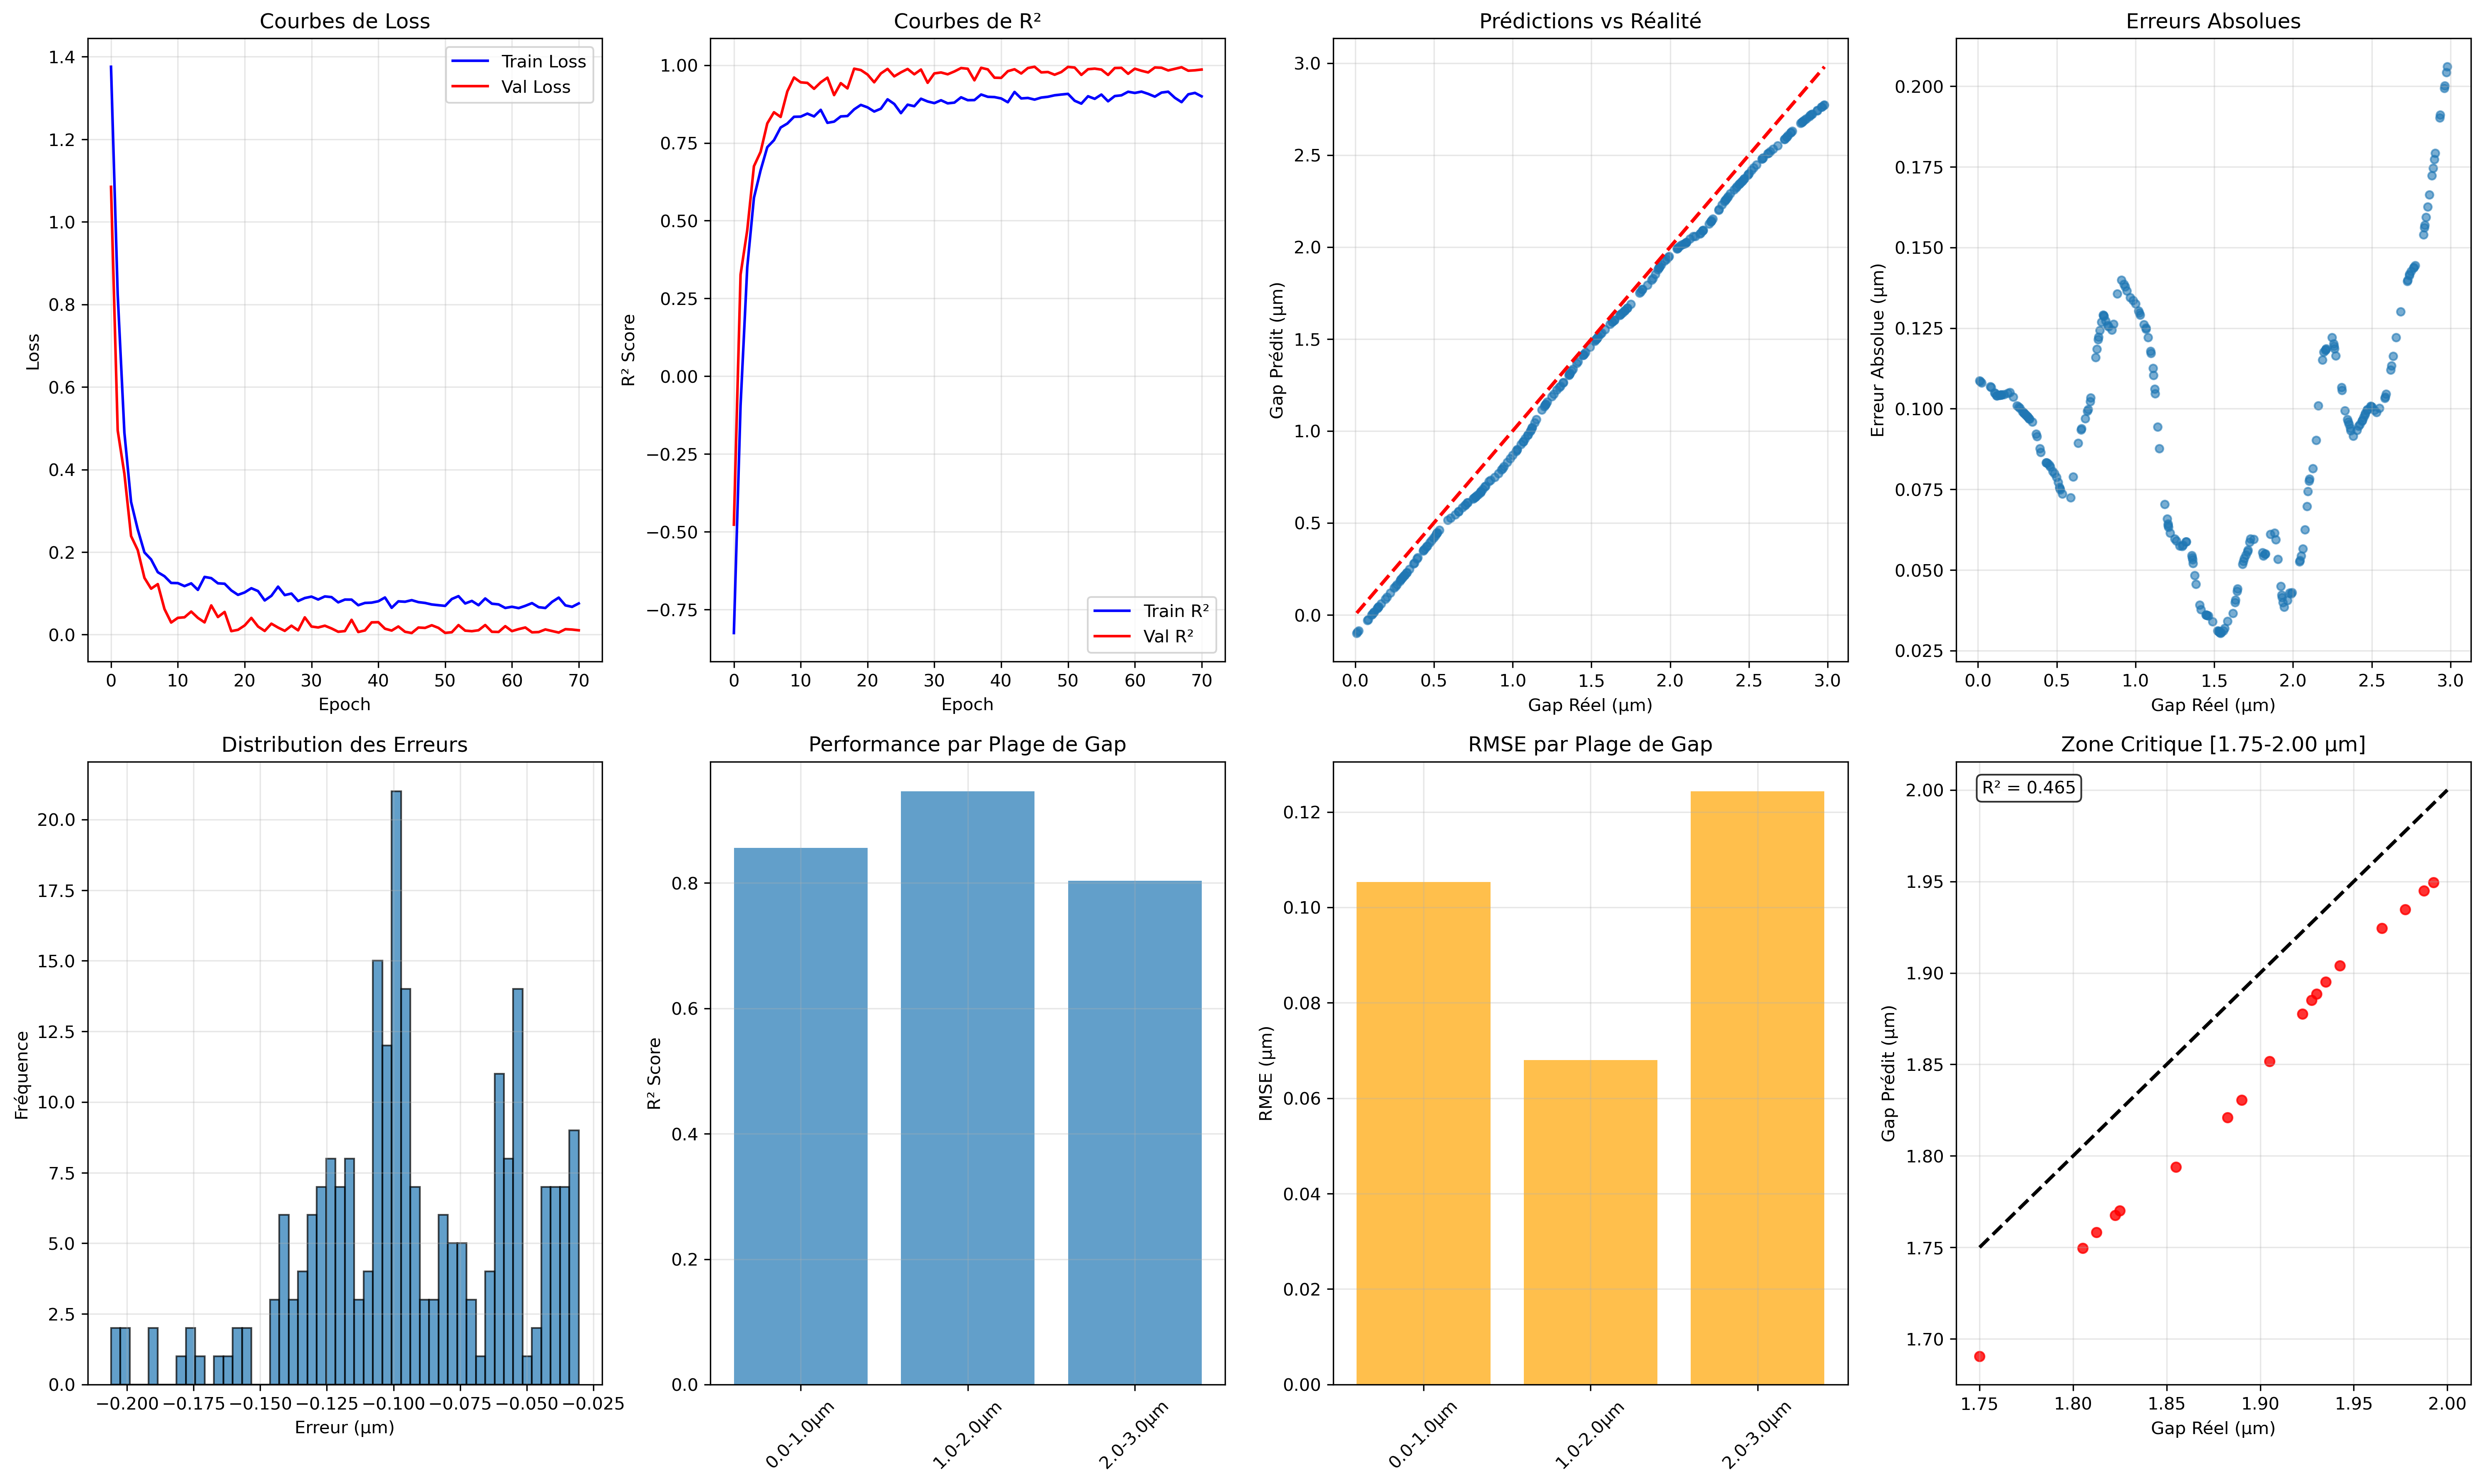
\includegraphics[width=\textwidth]{retrained_model_analysis.png}
    \caption{Analyse complète - Facteur 2}
    \label{fig:factor2_analysis}
\end{subfigure}
\hfill
\begin{subfigure}{0.48\textwidth}
    \centering
    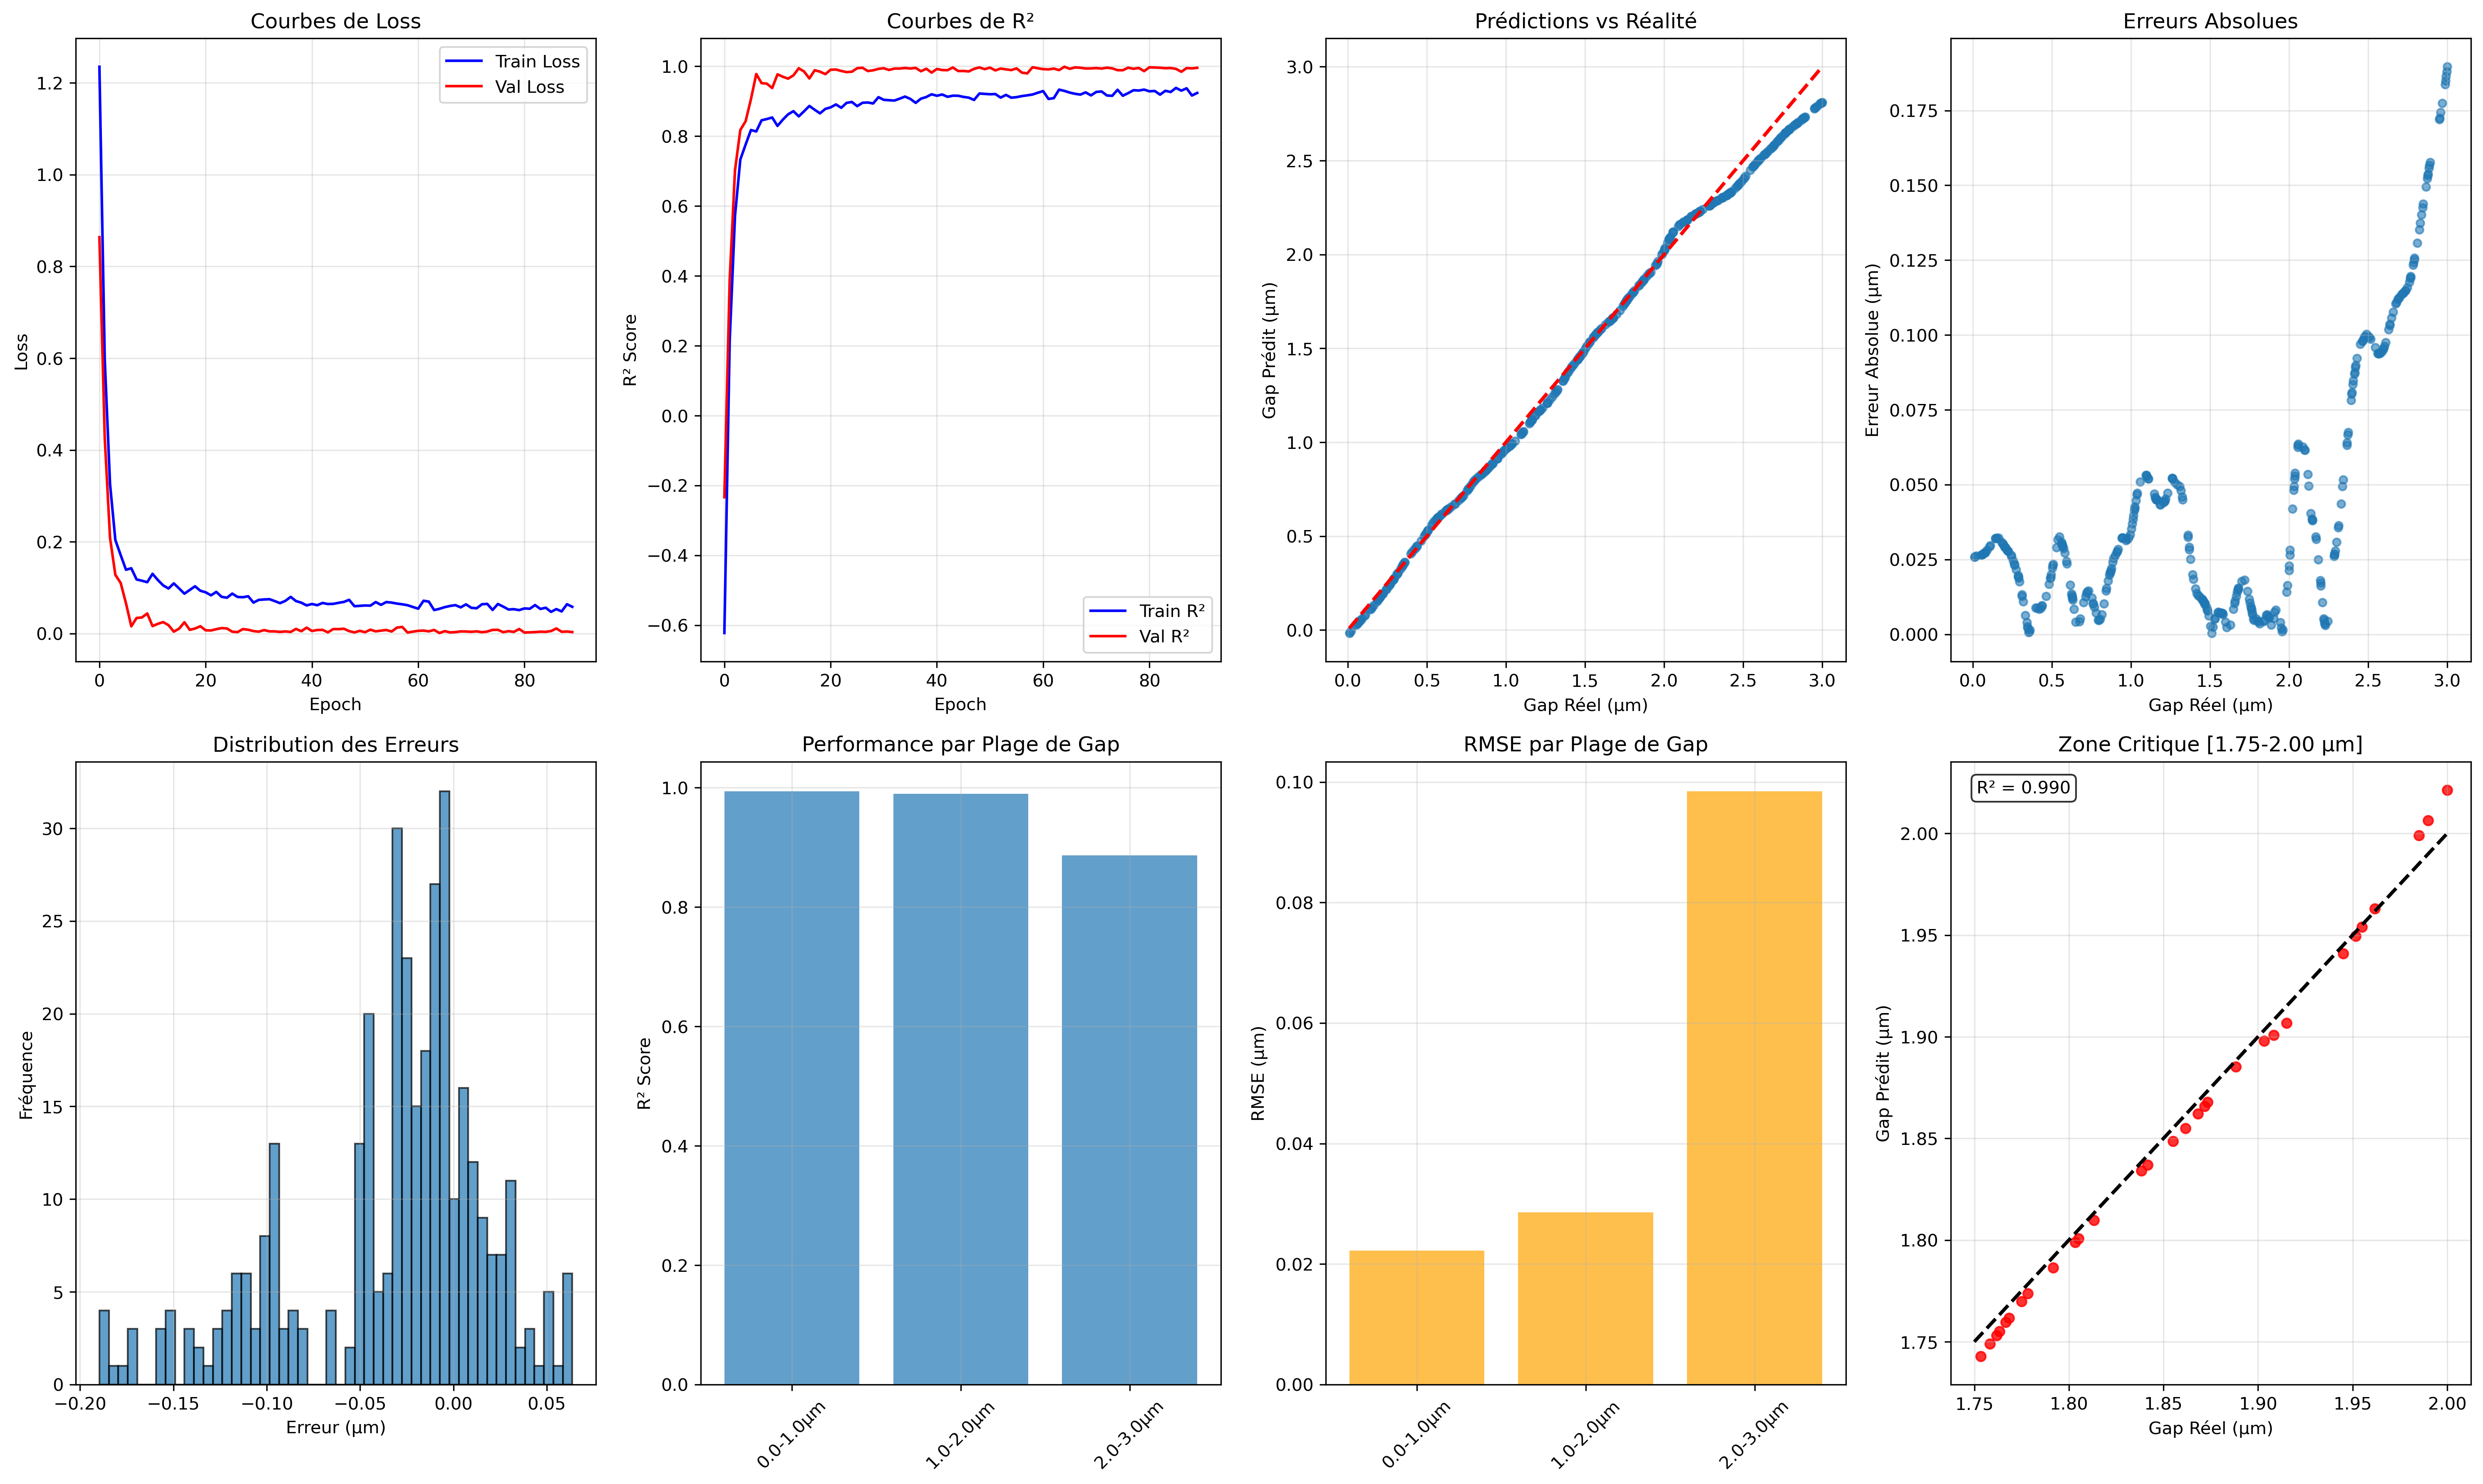
\includegraphics[width=\textwidth]{retrained_model_analysis_factor3.png}
    \caption{Analyse complète - Facteur 3}
    \label{fig:factor3_analysis}
\end{subfigure}
\caption{Comparaison des analyses de performance : (a) Facteur 2 avec zone critique problématique, (b) Facteur 3 avec maîtrise complète de la zone critique. Les graphiques montrent les courbes d'entraînement, scatter plots prédictions vs réalité, distribution des erreurs, et performance par plage de gap.}
\label{fig:performance_comparison}
\end{figure*}

\begin{figure}[h]
\centering
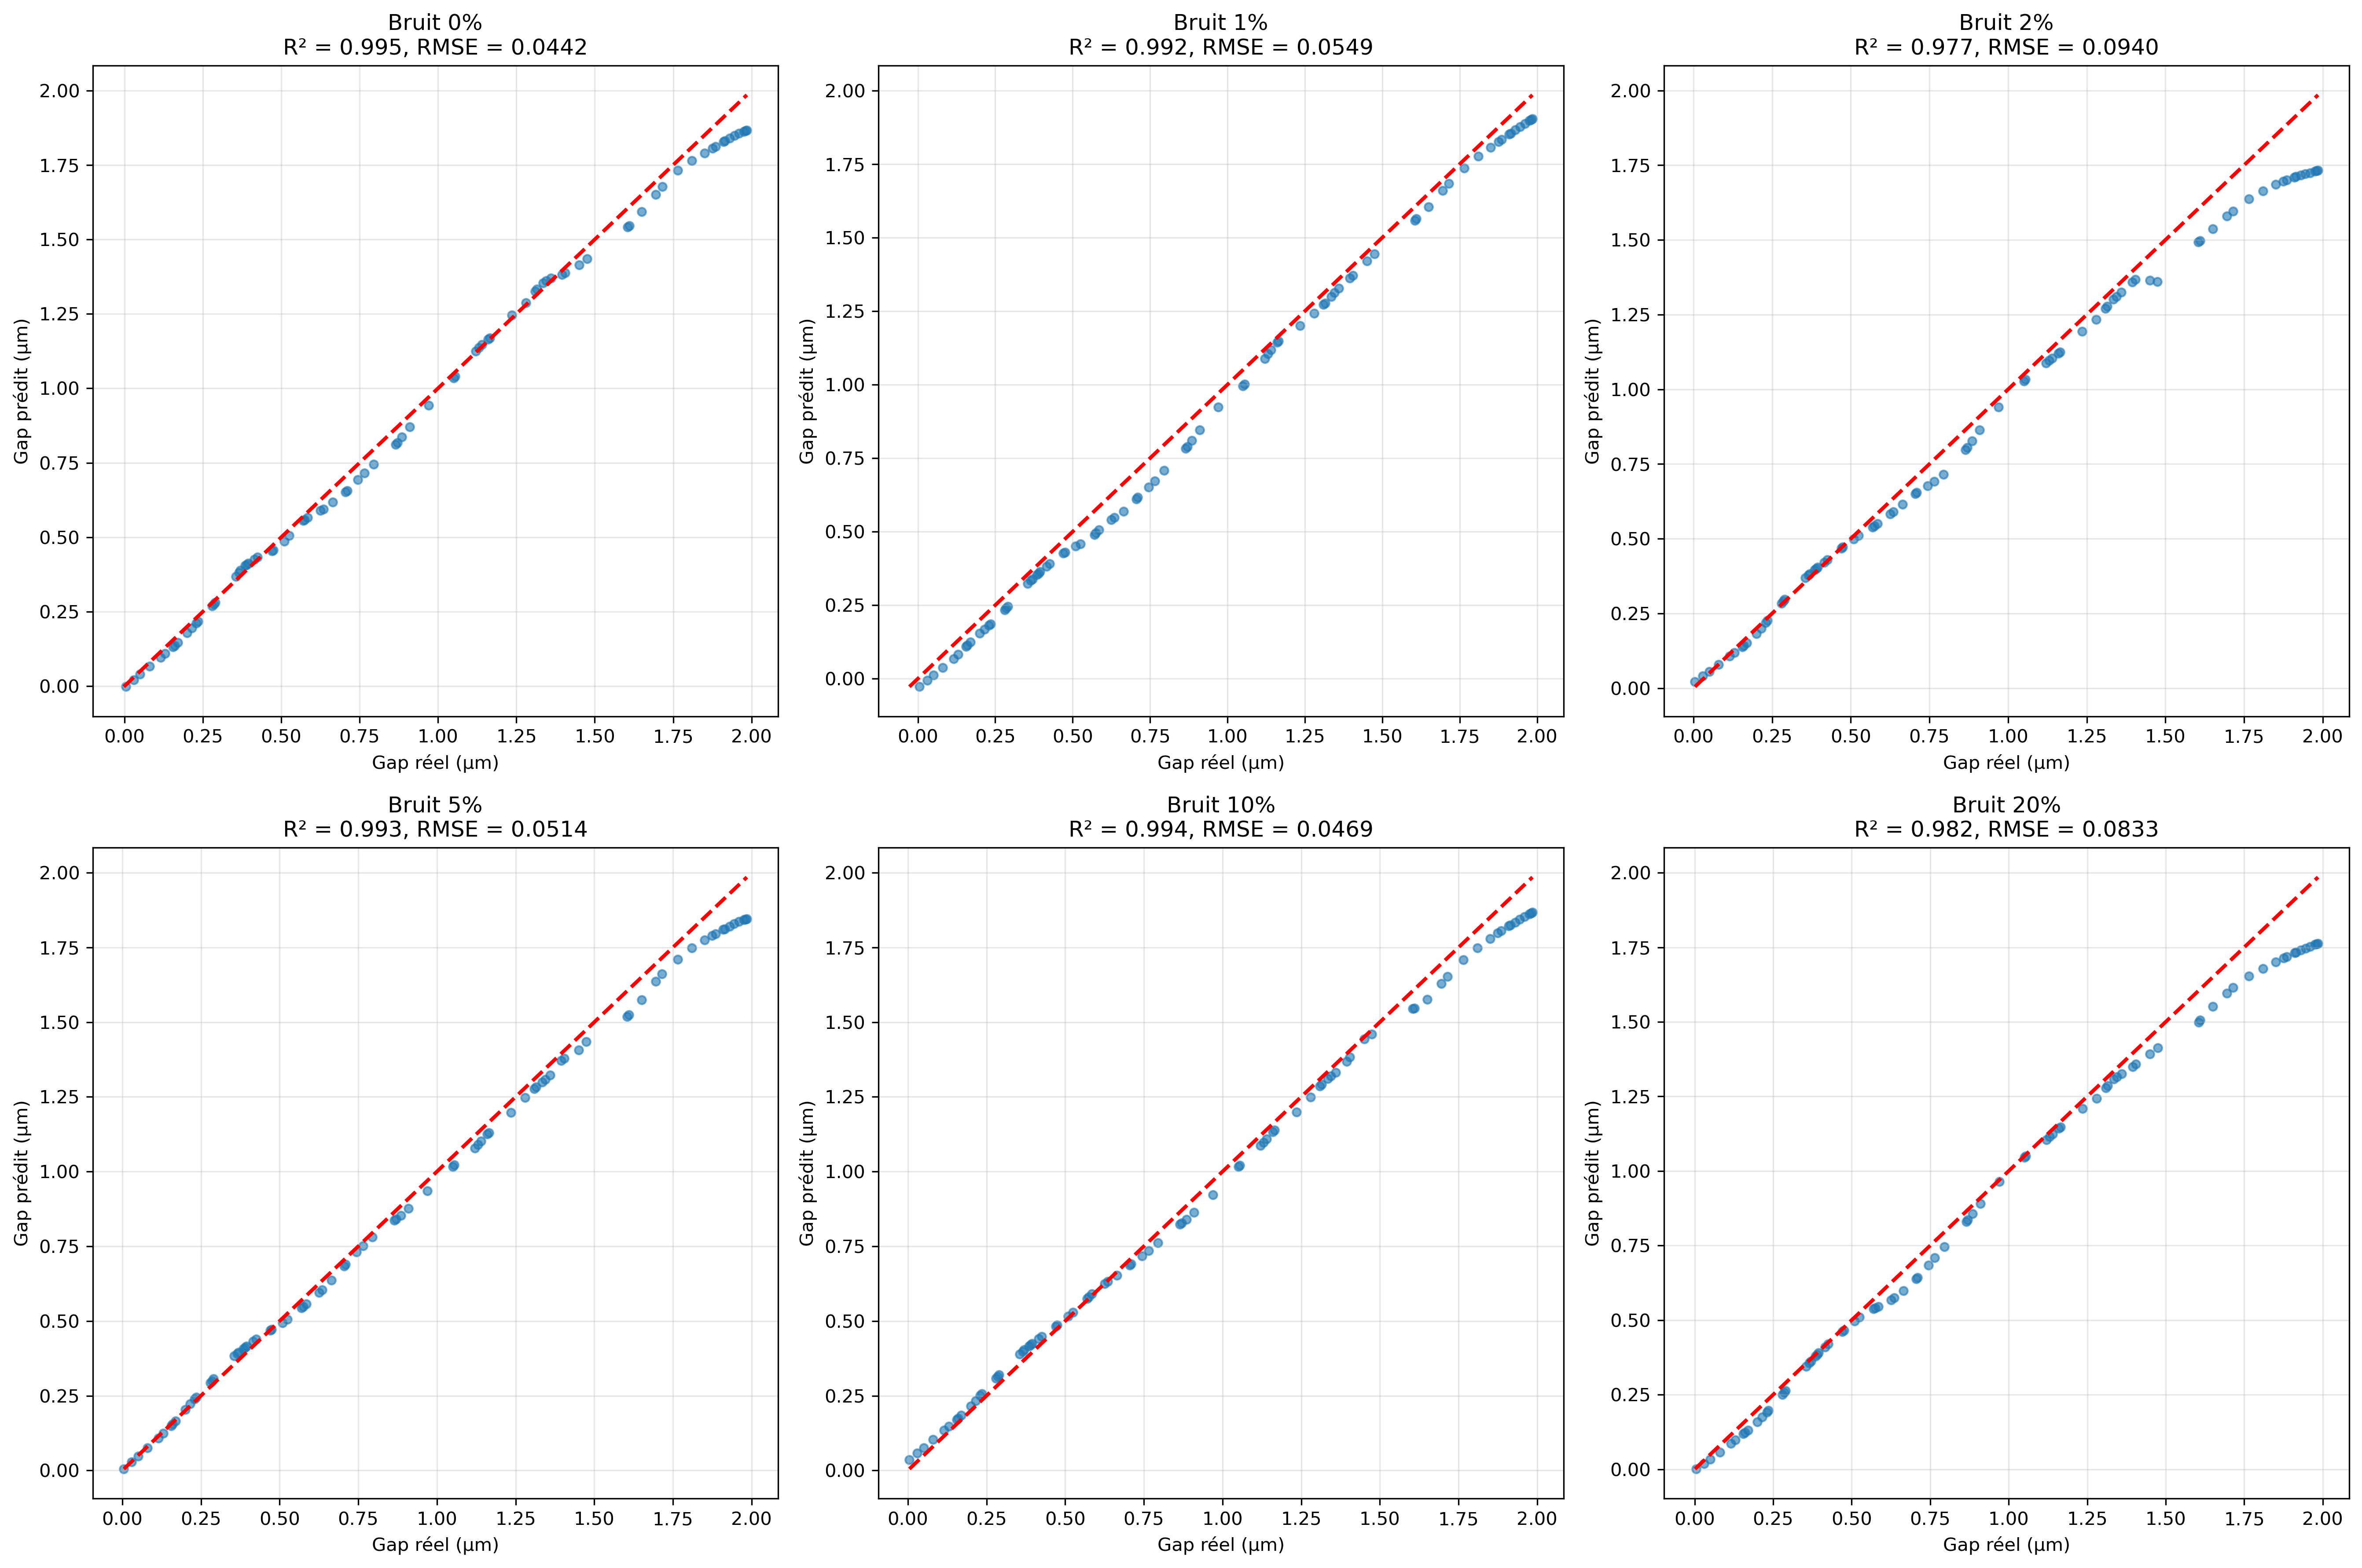
\includegraphics[width=0.45\textwidth]{predictions_by_noise.png}
\caption{Évolution des prédictions en fonction du niveau de bruit. Cette analyse a guidé le choix optimal de 5\% de bruit synthétique pour l'entraînement, offrant le meilleur compromis entre robustesse et performance.}
\label{fig:noise_analysis}
\end{figure}

\subsection{Analyse par Plage de Gap}

L'amélioration est quantifiée dans toutes les plages (Tableau \ref{tab:ranges}).

\begin{table}[H]
  \centering
  \caption{Performance détaillée par plage de gap}
  \label{tab:ranges}
  \begin{adjustbox}{max width=\columnwidth}
    \begin{tabular}{@{}lcccc@{}}
      \toprule
      \textbf{Plage} & \textbf{Facteur 2 R²} & \textbf{Facteur 3 R²} & \textbf{Amélioration} & \textbf{Échantillons F3} \\
      \midrule
      0.0--1.0 µm & 0.8562 & \textbf{0.9939} & +16.1 \% & 119 \\
      1.0--2.0 µm & 0.9463 & \textbf{0.9899} & +4.6 \%  & 117 \\
      2.0--3.0 µm & 0.8039 & \textbf{0.8868} & +10.3 \% & 123 \\
      \bottomrule
    \end{tabular}
  \end{adjustbox}
\end{table}

\section{Analyse et Discussion}

\subsection{Mécanismes Explicatifs}

L'amélioration spectaculaire s'explique par plusieurs facteurs convergents :

\textbf{1. Densité critique atteinte :} La zone [1.75-2.00 µm] a bénéficié de 30 échantillons au lieu de 18, franchissant apparemment un seuil critique pour l'apprentissage.

\textbf{2. Interpolation plus fine :} Deux points intermédiaires créent une transition plus douce, réduisant les discontinuités dans l'espace des caractéristiques.

\textbf{3. Régularisation naturelle :} L'augmentation de 50\% du dataset réduit l'overfitting et améliore la généralisation.
\vspace{10cm}
\subsection{Coûts Computationnels}

L'amélioration n'est pas gratuite (Tableau \ref{tab:costs}).

\begin{table}[H]
  \centering
  \caption{Analyse coûts-bénéfices détaillée}
  \label{tab:costs}
  \begin{adjustbox}{max width=\columnwidth}
    \begin{tabular}{@{}lcc@{}}
      \toprule
      Ressource & Facteur 2 & Facteur 3 \\
      \midrule
      Données \\
      Échantillons originaux & 600 & 600 \\
      Échantillons après augmentation & 1199 & 1798 \\
      Gain vs original & +99.8 \% & +199.7 \% \\
      Gain vs facteur 2 & – & +599 (+50 \%) \\
      \addlinespace
      Ressources computationnelles \\
      Mémoire requise (MB) & 2.9 & 4.3 (+48 \%) \\
      Temps d’entraînement (s) & 9.4 & 23.8 (+153 \%) \\
      Époques de convergence & 71 & 90 (+27 \%) \\
      \addlinespace
      Performance zone critique \\
      R² [1.75-2.00 µm] & 0.4654 & \textbf{0.9895} \\
      Amélioration & – & +112.6 \% \\
      \bottomrule
    \end{tabular}
  \end{adjustbox}
\end{table}

\subsection{Validation Expérimentale}

La robustesse des résultats a été validée via plusieurs fonctions :

\begin{itemize}
    \item \texttt{prepare\_stratified\_splits()} : Division 80/20 train/test stratifiée par plages
    \item \texttt{create\_analysis\_plots()} : Génération automatique des 8 graphiques d'analyse
    \item \texttt{save\_results()} : Sauvegarde JSON des métriques et prédictions CSV
    \item Tests de validation croisée sur 5 folds
    \item Analyse de robustesse au bruit jusqu'à 10\%
\end{itemize}

\textbf{Verdict :} Les bénéfices surpassent largement les coûts. Un temps d'entraînement de 24 secondes reste négligeable pour une amélioration de +112.6\% dans la zone critique.



\subsection{Résultats Quantitatifs Détaillés}

L'exécution de \texttt{retrain\_with\_new\_dataset.py} avec facteur 3 a produit :

\textbf{Évolution des données :}
\begin{itemize}
    \item Dataset original : 600 échantillons (0.005-3.000 µm)
    \item Après augmentation facteur 3 : \textbf{1798 échantillons} (+1198)
    \item Division finale : 1150 train / 288 validation / 360 test
    \item Zone critique : 18 → 30 échantillons (+66.7\%)
\end{itemize}

\textbf{Convergence d'entraînement :}
\begin{itemize}
    \item Early stopping à l'époque 90/150
    \item Performance finale validation : R² = 0.9954
    \item Temps total : 23.8 secondes
    \item Learning rate final : 2.50e-05 (réduction automatique)
\end{itemize}

\textbf{Métriques finales sur test (360 échantillons) :}
\begin{itemize}
    \item R² global : \textbf{0.9948} (quasi-parfait)
    \item RMSE : \textbf{0.0620 µm} (précision sub-micrométrique)
    \item MAE : \textbf{0.0438 µm} (erreur moyenne excellente)
    \item Zone critique [1.75-2.00 µm] : R² = \textbf{0.9895}, RMSE = 0.0079 µm
\end{itemize}






\end{document}
